\documentclass{beamer}
\usepackage{../../shared/styles/custom}
\usepackage{../../shared/styles/conventions}

\usepackage{grffile}
\usepackage{tikz}
\usetikzlibrary{matrix,positioning,backgrounds,fit,calc,arrows.meta,shapes}

\title{Matrix Factorization for Movie Recommendation Systems}
\date{\today}
\author{Nipun Batra}
\institute{IIT Gandhinagar}

\begin{document}
\maketitle

\begin{frame}{Today's Learning Journey}
\begin{itemize}[<+->]
    \item \textbf{The Problem}: Why do we need recommendation systems?
    \item \textbf{Matrix View}: How ratings become a mathematical problem
    \item \textbf{Key Insight}: Matrix factorization as the solution
    \item \textbf{Step-by-Step}: Building intuition with examples
    \item \textbf{Algorithms}: ALS vs Gradient Descent
    \item \textbf{Practice}: Hands-on understanding
\end{itemize}
\end{frame}

\section{Problem Setup}

\begin{frame}{The Movie Recommendation Challenge}
\begin{columns}[T]
\begin{column}{0.5\textwidth}
\textbf{Real-World Scenario:}
\begin{itemize}[<+->]
    \item Netflix: 200M+ users, 15K+ titles
    \item Most ratings are missing!
\end{itemize}

\pause
\vspace{0.3cm}
\textbf{The Challenge:}
\begin{itemize}[<+->]
    \item You've rated ~100 movies out of 15,000
    \item How do we predict what you'll like?
\end{itemize}
\end{column}
\begin{column}{0.5\textwidth}
\only<4->{
\begin{center}
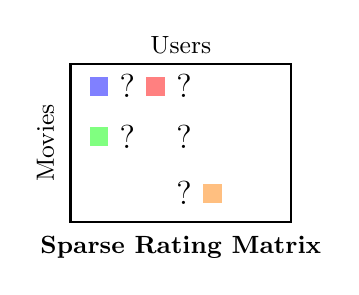
\begin{tikzpicture}[scale=0.8]
    \draw[thick] (0,0) rectangle (3.5,2.5);
    \node at (1.75,2.8) {\small Users};
    \node[rotate=90] at (-0.4,1.25) {\small Movies};
    
    % Some filled squares (known ratings)
    \fill[blue!50] (0.3,2) rectangle (0.6,2.3);
    \fill[red!50] (1.2,2) rectangle (1.5,2.3);
    \fill[green!50] (0.3,1.2) rectangle (0.6,1.5);
    \fill[orange!50] (2.1,0.3) rectangle (2.4,0.6);
    
    % Question marks for missing (fewer to reduce clutter)
    \node at (0.9,2.15) {\large ?};
    \node at (1.8,2.15) {\large ?};
    \node at (0.9,1.35) {\large ?};
    \node at (1.8,1.35) {\large ?};
    \node at (1.8,0.45) {\large ?};
    
    \node at (1.75,-0.4) {\small \textbf{Sparse Rating Matrix}};
\end{tikzpicture}
\end{center}
}
\end{column}
\end{columns}
\end{frame}

\stepcounter{popquiz}
\begin{frame}{Pop Quiz \#\thepopquiz: Understanding the Scale}
\begin{popquizbox}{\thepopquiz}
If Netflix has 200 million users and 15,000 movies, how many possible ratings exist?

\textbf{Hint:} Think about the total number of user-movie pairs
\end{popquizbox}
\end{frame}

\begin{frame}{Pop Quiz \#\thepopquiz: Understanding the Scale - Answer}
\begin{popquizbox}{\thepopquiz}
\textbf{Answer:} $200 \times 10^6 \times 15 \times 10^3 = 3 \times 10^{12}$ possible ratings!

\textbf{Follow-up:} If typical users rate only 100 movies, what percentage of the matrix is filled?

\textbf{Answer:} $\frac{100}{15000} = 0.67\%$ - extremely sparse!
\end{popquizbox}

\pause
\begin{alertbox}{The Sparsity Challenge}
99.33\% of the rating matrix is empty! This is why we need smart algorithms.
\end{alertbox}
\end{frame}

\begin{frame}{Mathematical Problem Setup}
\textbf{The Rating Matrix} $\mA \in \Real^{N \times M}$ with proper labels:

\pause
\begin{center}
\renewcommand{\arraystretch}{1.3}
\begin{tabular}{c|ccccc}
 & \textbf{Sholay} & \textbf{Swades} & \textbf{Batman} & \textbf{Interstellar} & \textbf{...} \\
\hline
\textbf{Arjun} & $a_{11}$ & ? & $a_{13}$ & ? & $\cdots$ \\
\textbf{Priya} & ? & $a_{22}$ & ? & $a_{24}$ & $\cdots$ \\
\textbf{Ravi} & $a_{31}$ & ? & ? & $a_{34}$ & $\cdots$ \\
\textbf{...} & $\vdots$ & $\vdots$ & $\vdots$ & $\vdots$ & $\ddots$
\end{tabular}
\end{center}

\pause
\begin{itemize}[<+->]
    \item \textbf{Rows}: Users $u_1 = \text{Arjun}, u_2 = \text{Priya}, u_3 = \text{Ravi}, \ldots, u_N$ 
    \item \textbf{Columns}: Movies $m_1 = \text{Sholay}, m_2 = \text{Swades}, \ldots, m_M$
    \item \textbf{Entries}: $a_{ij} \in \{1,2,3,4,5\}$ (when observed)
    \item \textbf{Challenge}: Predict missing entries $?$
    \item \textbf{Notation}: $\Omega = \{(i,j) : a_{ij} \text{ is observed}\}$
\end{itemize}
\end{frame}

\begin{frame}{Concrete Example: Our Movie Dataset}
Let's work with a small, concrete example:

\pause
\begin{center}
\renewcommand{\arraystretch}{1.2}
\begin{tabular}{l|ccccc}
\toprule
\textbf{User} & \textbf{Sholay} & \textbf{Swades} & \textbf{Batman} & \textbf{Interstellar} & \textbf{Shawshank} \\
\midrule
Arjun & \textcolor{blue}{5} & \textcolor{blue}{4} & \textcolor{red}{2} & \textcolor{red}{3} & \textcolor{red}{2} \\
Priya & \textcolor{red}{?} & \textcolor{blue}{5} & \textcolor{red}{1} & \textcolor{blue}{4} & \textcolor{red}{?} \\
Ravi & \textcolor{blue}{4} & \textcolor{red}{?} & \textcolor{red}{1} & \textcolor{blue}{5} & \textcolor{red}{?} \\
\bottomrule
\end{tabular}
\end{center}

\pause
\textbf{Observations:}
\begin{itemize}[<+->]
    \item Arjun loves Bollywood films (Sholay, Swades) 
    \item Ravi enjoys Sci-Fi (Interstellar)  
    \item Can we predict Priya's rating for Sholay?
    \item Can we predict Ravi's rating for Swades?
\end{itemize}
\end{frame}

\section{Key Insight: Latent Features}

\begin{frame}{Before We Dive In: A Simple Question}
\begin{center}
\Large \textbf{Why do you like the movies you like?}
\end{center}

\pause
\begin{columns}[T]
\begin{column}{0.5\textwidth}
\textbf{Maybe because of:}
\begin{itemize}[<+->]
    \item Genre (Action, Romance, Comedy)
    \item Star cast (Shah Rukh Khan, Tom Cruise)
    \item Director (Christopher Nolan, Rajkumar Hirani)
    \item Language (Hindi, English, Tamil)
    \item Era (90s classics, modern CGI)
\end{itemize}
\end{column}
\begin{column}{0.5\textwidth}
\only<6->{
\textbf{Key Insight:}
\begin{itemize}
    \item Your taste = combination of preferences
    \item Movie appeal = combination of features
    \item \textcolor{red}{But we don't know these explicitly!}
\end{itemize}
}
\end{column}
\end{columns}
\end{frame}

\begin{frame}{The Core Insight: Hidden Patterns}
\begin{columns}[T]
\begin{column}{0.6\textwidth}
\textbf{Hypothesis:} User preferences and movie characteristics can be captured by a small number of \textbf{latent features}.

\pause
\textbf{Intuition:} Think of latent features as "hidden DNA" of movies and users!

\pause
\vspace{0.5cm}
\textbf{For Movies:}
\begin{itemize}[<+->]
    \item Bollywood vs Hollywood
    \item Action vs Drama  
    \item Comedy vs Serious
    \item Runtime (Short vs Long)
    \item Year (Classic vs Modern)
\end{itemize}
\end{column}
\begin{column}{0.4\textwidth}
\only<6->{
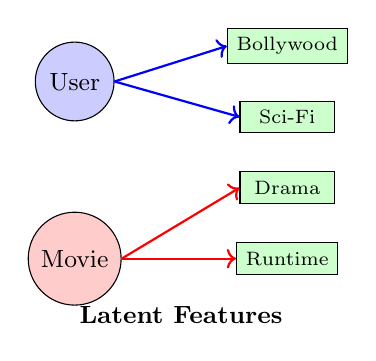
\begin{tikzpicture}[scale=0.9]
    \node[draw, circle, fill=blue!20, minimum size=1cm] (user) at (0,2.5) {\small User};
    \node[draw, circle, fill=red!20, minimum size=1cm] (movie) at (0,0) {\small Movie};
    
    \node[draw, rectangle, fill=green!20, minimum width=1.2cm] (f1) at (3,3) {\scriptsize Bollywood};
    \node[draw, rectangle, fill=green!20, minimum width=1.2cm] (f2) at (3,2) {\scriptsize Sci-Fi};
    \node[draw, rectangle, fill=green!20, minimum width=1.2cm] (f3) at (3,1) {\scriptsize Drama};
    \node[draw, rectangle, fill=green!20, minimum width=1.2cm] (f4) at (3,0) {\scriptsize Runtime};
    
    \draw[->, thick, blue] (user.east) -- (f1.west);
    \draw[->, thick, blue] (user.east) -- (f2.west);
    \draw[->, thick, red] (movie.east) -- (f3.west);
    \draw[->, thick, red] (movie.east) -- (f4.west);
    
    \node at (1.5,-0.8) {\small \textbf{Latent Features}};
\end{tikzpicture}
}
\end{column}
\end{columns}
\end{frame}

\begin{frame}{Step 1: Define Movie Features Explicitly}
Let's manually define features for our 5 movies:

\pause
\begin{center}
\renewcommand{\arraystretch}{1.3}
\begin{tabular}{l|ccc}
\toprule
\textbf{Movie} & \textbf{Bollywood} & \textbf{Sci-Fi} & \textbf{Drama} \\
\midrule
Sholay & \textcolor{blue}{0.95} & \textcolor{red}{0.10} & \textcolor{orange}{0.85} \\
Swades & \textcolor{blue}{1.00} & \textcolor{red}{0.20} & \textcolor{orange}{0.90} \\
Batman & \textcolor{blue}{0.05} & \textcolor{red}{0.80} & \textcolor{orange}{0.30} \\
Interstellar & \textcolor{blue}{0.05} & \textcolor{red}{0.95} & \textcolor{orange}{0.70} \\
Shawshank & \textcolor{blue}{0.05} & \textcolor{red}{0.15} & \textcolor{orange}{0.95} \\
\bottomrule
\end{tabular}
\end{center}

\pause
\textbf{Movie Feature Matrix} $\mH \in \Real^{3 \times 5}$:
\begin{equation*}
\mH = \begin{bmatrix}
\textcolor{blue}{0.95} & \textcolor{blue}{1.00} & \textcolor{blue}{0.05} & \textcolor{blue}{0.05} & \textcolor{blue}{0.05} \\
\textcolor{red}{0.10} & \textcolor{red}{0.20} & \textcolor{red}{0.80} & \textcolor{red}{0.95} & \textcolor{red}{0.15} \\
\textcolor{orange}{0.85} & \textcolor{orange}{0.90} & \textcolor{orange}{0.30} & \textcolor{orange}{0.70} & \textcolor{orange}{0.95}
\end{bmatrix}
\end{equation*}
\end{frame}

\begin{frame}{Step 2: What About User Preferences?}
\textbf{User Feature Matrix} $\mW \in \Real^{3 \times 3}$ represents user preferences:

\pause
\begin{center}
\renewcommand{\arraystretch}{1.4}
\begin{tabular}{c|ccc}
 & \textbf{Bollywood} & \textbf{Sci-Fi} & \textbf{Drama} \\
\hline
\textbf{Arjun} & \textcolor{blue}{3.8} & \textcolor{red}{0.8} & \textcolor{orange}{1.5} \\
\textbf{Priya} & \textcolor{blue}{1.8} & \textcolor{red}{4.1} & \textcolor{orange}{3.2} \\
\textbf{Ravi} & \textcolor{blue}{2.4} & \textcolor{red}{4.8} & \textcolor{orange}{2.1}
\end{tabular}
\end{center}

\pause
\textbf{Each row = one user's preference profile}

\pause
\textbf{Next:} Let's understand what each number means!
\end{frame}

\begin{frame}{User Preference Interpretation}
\textbf{What do these numbers tell us?}

\pause
\begin{center}
\renewcommand{\arraystretch}{1.6}
\begin{tabular}{c|ccc}
 & \textbf{Bollywood} & \textbf{Sci-Fi} & \textbf{Drama} \\
\hline
\textbf{Arjun} & \textcolor{blue}{3.8} & \textcolor{red}{0.8} & \textcolor{orange}{1.5} \\
\textbf{Priya} & \textcolor{blue}{1.8} & \textcolor{red}{4.1} & \textcolor{orange}{3.2} \\
\textbf{Ravi} & \textcolor{blue}{2.4} & \textcolor{red}{4.8} & \textcolor{orange}{2.1}
\end{tabular}
\end{center}

\pause
\begin{itemize}[<+->]
    \item \textbf{Arjun:} Strong Bollywood fan, weak Sci-Fi
    \item \textbf{Priya:} Strong Sci-Fi fan, moderate Drama
    \item \textbf{Ravi:} Very strong Sci-Fi fan
\end{itemize}

\pause
\textbf{The Magic:} These values × movie features should recreate observed ratings!
\end{frame}

\begin{frame}{Focus: Arjun's Bollywood Preference}
\textbf{Understanding $w_{11}$ - how much Arjun likes Bollywood:}

\pause
\begin{center}
\renewcommand{\arraystretch}{1.6}
\begin{tabular}{c|ccc}
 & \textbf{Bollywood} & \textbf{Sci-Fi} & \textbf{Drama} \\
\hline
\textbf{Arjun} & \cellcolor{red!50}\textcolor{blue}{3.8} & \textcolor{red}{0.8} & \textcolor{orange}{1.5} \\
\textbf{Priya} & \textcolor{blue}{1.8} & \textcolor{red}{4.1} & \textcolor{orange}{3.2} \\
\textbf{Ravi} & \textcolor{blue}{2.4} & \textcolor{red}{4.8} & \textcolor{orange}{2.1}
\end{tabular}
\end{center}

\pause
\textcolor{red}{\textbf{$w_{11} = 3.8$}}: Arjun's strong Bollywood preference!

\pause
This explains why he gave Sholay (high Bollywood content) a rating of 5.
\end{frame}

\begin{frame}{Focus: Arjun's Sci-Fi Preference}
\textbf{Understanding $w_{12}$ - how much Arjun likes Sci-Fi:}

\pause
\begin{center}
\renewcommand{\arraystretch}{1.6}
\begin{tabular}{c|ccc}
 & \textbf{Bollywood} & \textbf{Sci-Fi} & \textbf{Drama} \\
\hline
\textbf{Arjun} & \textcolor{blue}{3.8} & \cellcolor{blue!50}\textcolor{red}{0.8} & \textcolor{orange}{1.5} \\
\textbf{Priya} & \textcolor{blue}{1.8} & \textcolor{red}{4.1} & \textcolor{orange}{3.2} \\
\textbf{Ravi} & \textcolor{blue}{2.4} & \textcolor{red}{4.8} & \textcolor{orange}{2.1}
\end{tabular}
\end{center}

\pause
\textcolor{blue}{\textbf{$w_{12} = 0.8$}}: Arjun's weak Sci-Fi preference

\pause
This explains why he gave Interstellar (high Sci-Fi) only a rating of 3.
\end{frame}

\begin{frame}{Focus: Arjun's Drama Preference}
\textbf{Understanding $w_{13}$ - how much Arjun likes Drama:}

\pause
\begin{center}
\renewcommand{\arraystretch}{1.6}
\begin{tabular}{c|ccc}
 & \textbf{Bollywood} & \textbf{Sci-Fi} & \textbf{Drama} \\
\hline
\textbf{Arjun} & \textcolor{blue}{3.8} & \textcolor{red}{0.8} & \cellcolor{green!50}\textcolor{orange}{1.5} \\
\textbf{Priya} & \textcolor{blue}{1.8} & \textcolor{red}{4.1} & \textcolor{orange}{3.2} \\
\textbf{Ravi} & \textcolor{blue}{2.4} & \textcolor{red}{4.8} & \textcolor{orange}{2.1}
\end{tabular}
\end{center}

\pause
\textcolor{green}{\textbf{$w_{13} = 1.5$}}: Arjun's low Drama preference

\pause
This explains why he gave Shawshank (high Drama) only a rating of 2.
\end{frame}

\begin{frame}{Arjun's Complete Taste Profile}
\textbf{Putting it all together:}

\pause
\begin{center}
\renewcommand{\arraystretch}{1.6}
\begin{tabular}{c|ccc}
 & \textbf{Bollywood} & \textbf{Sci-Fi} & \textbf{Drama} \\
\hline
\textbf{Arjun} & \cellcolor{red!30}\textcolor{blue}{3.8} & \cellcolor{blue!30}\textcolor{red}{0.8} & \cellcolor{green!30}\textcolor{orange}{1.5} \\
\textbf{Priya} & \textcolor{blue}{1.8} & \textcolor{red}{4.1} & \textcolor{orange}{3.2} \\
\textbf{Ravi} & \textcolor{blue}{2.4} & \textcolor{red}{4.8} & \textcolor{orange}{2.1}
\end{tabular}
\end{center}

\pause
\begin{keypointsbox}{}
Arjun's taste profile: [\textcolor{red}{3.8 Bollywood}, \textcolor{blue}{0.8 Sci-Fi}, \textcolor{green}{1.5 Drama}]
\end{keypointsbox}
\end{frame}

\begin{frame}{Step 3: The Matrix Factorization Idea}
\textbf{Core Hypothesis:} Rating = User preferences · Movie features

\pause
\begin{equation*}
\boxed{a_{ij} \approx \vw_i^T \vh_j = \sum_{k=1}^r w_{ik} h_{kj}}
\end{equation*}

\pause
\textbf{In Matrix Form:}
\begin{equation*}
\boxed{\mA \approx \mW \mH}
\end{equation*}

\pause
\begin{center}
$\mA_{3 \times 5} =
\begin{bmatrix}
5 & 4 & 2 & 3 & 2 \\
? & 5 & 1 & 4 & ? \\
4 & ? & 1 & 5 & ? 
\end{bmatrix}
\approx
\begin{bmatrix}
3.8 & 0.8 & 1.5 \\
1.8 & 4.1 & 3.2 \\
2.4 & 4.8 & 2.1
\end{bmatrix}
\begin{bmatrix}
0.95 & 1.00 & 0.05 & 0.05 & 0.05 \\
0.10 & 0.20 & 0.80 & 0.95 & 0.15 \\
0.85 & 0.90 & 0.30 & 0.70 & 0.95
\end{bmatrix}
= \mW_{3 \times 3} \mH_{3 \times 5}$
\end{center}
\end{frame}

\begin{frame}{Step 4: Understanding the Calculation}
\textbf{Let's predict Arjun's rating for Sholay step by step...}

\pause
\begin{columns}[T]
\begin{column}{0.5\textwidth}
\textbf{Arjun's Profile:}
\begin{itemize}[<+->]
    \item How much does he like Bollywood? \textcolor{red}{$w_{11} = 3.8$}
    \item How much does he like Sci-Fi? \textcolor{blue}{$w_{12} = 0.8$}
    \item How much does he like Drama? \textcolor{green}{$w_{13} = 1.5$}
\end{itemize}
\end{column}
\begin{column}{0.5\textwidth}
\only<4->{
\textbf{Sholay's DNA:}
\begin{itemize}
    \item Bollywood-ness: \textcolor{red}{0.95} (very high!)
    \item Sci-Fi-ness: \textcolor{blue}{0.10} (low)
    \item Drama-ness: \textcolor{green}{0.85} (high)
\end{itemize}
}
\end{column}
\end{columns}

\pause
\vspace{0.5cm}
\textbf{The Magic Formula:} 
$$\text{Arjun's rating} = \text{Arjun's preferences} \cdot \text{Sholay's features}$$
\end{frame}

\begin{frame}{Step 4: Detailed Calculation Example}
Let's compute Arjun's predicted rating for Sholay:

\pause
\textbf{Arjun's preferences:} $\vw_1 = [\textcolor{red}{3.8}, \textcolor{blue}{0.8}, \textcolor{green}{1.5}]$

\textbf{Sholay's features:} $\vh_1 = [\textcolor{red}{0.95}, \textcolor{blue}{0.10}, \textcolor{green}{0.85}]^T$

\pause
\begin{align}
\hat{a}_{11} &= \vw_1^T \vh_1 \\
&= \textcolor{red}{3.8 \cdot 0.95} + \textcolor{blue}{0.8 \cdot 0.10} + \textcolor{green}{1.5 \cdot 0.85} \\
&= \textcolor{red}{3.61} + \textcolor{blue}{0.08} + \textcolor{green}{1.28} = \textbf{4.97}
\end{align}

\pause $\hat{a}_{11} = 4.97 \approx 5$ $\checkmark$ 

This shows how matrix factorization works: find user preferences that recreate observed ratings!
\end{frame}

\stepcounter{popquiz}
\begin{frame}{Pop Quiz \#\thepopquiz: Matrix Dimensions}
\begin{popquizbox}{\thepopquiz}
If we have $N$ users, $M$ movies, and $r$ latent features:

\pause
\begin{enumerate}[<+->]
    \item What are the dimensions of $\mA$? 
    \item What are the dimensions of $\mW$?
    \item What are the dimensions of $\mH$?
    \item How many parameters do we need to learn?
\end{enumerate}
\end{popquizbox}
\end{frame}

\begin{frame}{Pop Quiz \#\thepopquiz: Matrix Dimensions - Answers}
\begin{popquizbox}{\thepopquiz}
\textbf{Answers:}
\begin{enumerate}
    \item $\mA \in \Real^{N \times M}$ (rating matrix)
    \item $\mW \in \Real^{N \times r}$ (user preferences)
    \item $\mH \in \Real^{r \times M}$ (movie features)
    \item Total parameters: $Nr + rM = r(N + M)$
\end{enumerate}

\pause
\begin{keypointsbox}{}
If $r \ll \min(N,M)$, we have huge parameter reduction!
\end{keypointsbox}
\end{popquizbox}
\end{frame}

\section{Learning the Factorization}

\begin{frame}{The Optimization Problem}
\textbf{Objective:} Minimize prediction error on observed ratings only

\pause
\begin{equation*}
\boxed{\minimize_{\mW,\mH} \sum_{(i,j) \in \Omega} (a_{ij} - \vw_i^T \vh_j)^2}
\end{equation*}

\pause
\textbf{In Matrix Notation:}
\begin{equation*}
\boxed{\minimize_{\mW,\mH} \|P_\Omega(\mA - \mW\mH)\|_F^2}
\end{equation*}

\pause
Where:
\begin{itemize}[<+->]
    \item $P_\Omega(\cdot)$: only consider entries where we have ratings
    \item $\|\cdot\|_F$: Frobenius norm
    \item $\Omega$: set of observed $(i,j)$ pairs
\end{itemize}
\end{frame}

\begin{frame}{Why This is Challenging}
\textbf{Problem Characteristics:}
\begin{itemize}[<+->]
    \item \textbf{Non-convex:} Multiple local minima exist
    \item \textbf{Bilinear:} Linear in $\mW$ when $\mH$ fixed, and vice versa
    \item \textbf{Large-scale:} Millions of users and items
    \item \textbf{Sparse:} Only 0.1-1\% of entries observed
\end{itemize}

\pause
\textbf{Key Insight:} While non-convex jointly, it's convex in each matrix individually!
\end{frame}


\section{Alternating Least Squares (ALS): A Visual Derivation}

\begin{frame}[fragile]{Step 0: Recap of Standard Least Squares}
\textbf{Objective:} Estimate $\vtheta \in \mathbb{R}^{d \times 1}$ from data matrix $\mX \in \mathbb{R}^{n \times d}$ and label vector $\vy \in \mathbb{R}^{n \times 1}$.

\begin{equation*}
\vy \approx \mX \vtheta \quad \Rightarrow \quad \hat{\vtheta} = \arg\min_{\vtheta} \|\vy - \mX \vtheta\|_2^2
\end{equation*}

\vspace{0.8em}

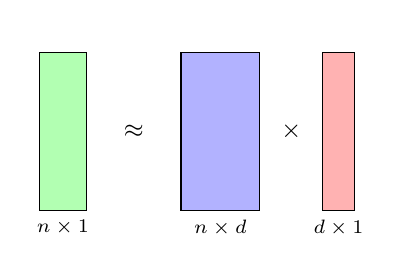
\begin{tikzpicture}[scale=1.0, every node/.style={font=\small}]
  \draw[fill=green!30] (-1.8,0) rectangle (-1.2,2);
  \node at (-1.5,2.2) {$\vy$};
  \node[below] at (-1.5,0) {\scriptsize $n \times 1$};

  \node at (-0.6,1) {$\approx$};

  \draw[fill=blue!30] (0.0,0) rectangle (1.0,2);
  \node at (0.5,2.2) {$\mX$};
  \node[below] at (0.5,0) {\scriptsize $n \times d$};

  \node at (1.4,1) {$\times$};

  \draw[fill=red!30] (1.8,0) rectangle (2.2,2);
  \node at (2.0,2.2) {$\vtheta$};
  \node[below] at (2.0,0) {\scriptsize $d \times 1$};
\end{tikzpicture}

\vspace{0.5em}
\textbf{Solution:} $\hat{\vtheta} = (\mX^\top \mX)^{-1} \mX^\top \vy$
\end{frame}


\begin{frame}[fragile]{ALS Problem Setup}
\textbf{Goal:} Decompose $\mA \in \mathbb{R}^{n \times m}$ as $\mW \mH$ with:

\begin{align*}
  \mW &\in \mathbb{R}^{n \times k} \\
  \mH &\in \mathbb{R}^{k \times m}
\end{align*}

\vspace{0.5em}
\textbf{Objective:} $\mA \approx \mW \mH$ with $k \ll \min(n, m)$

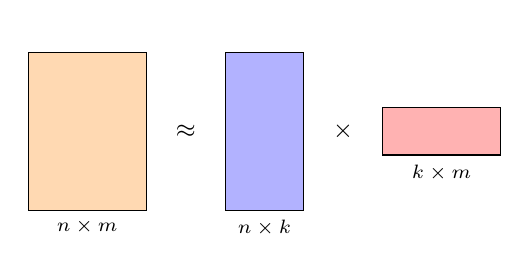
\begin{tikzpicture}[scale=1.0, every node/.style={font=\small}]
  \draw[fill=orange!30] (0,0) rectangle (1.5,2);
  \node at (0.75,2.2) {$\mA$};
  \node[below] at (0.75,0) {\scriptsize $n \times m$};

  \node at (2.0,1.0) {$\approx$};

  \draw[fill=blue!30] (2.5,0) rectangle (3.5,2);
  \node at (3.0,2.2) {$\mW$};
  \node[below] at (3.0,0) {\scriptsize $n \times k$};

  \node at (4.0,1.0) {$\times$};

  \draw[fill=red!30] (4.5,0.7) rectangle (6.0,1.3);
  \node at (5.25,1.5) {$\mH$};
  \node[below] at (5.25,0.7) {\scriptsize $k \times m$};
\end{tikzpicture}

\vspace{0.5em}
\textbf{Challenge:} Both $\mW$ and $\mH$ are unknown.
\end{frame}


\begin{frame}[fragile]{Step 1: Fix $\mW$, Learn $\mH$ One Column at a Time}
\textbf{Idea:} With $\mW$ fixed, each column of $\mH$ can be estimated via LS.

\begin{align*}
  \mA[:, j] &\approx \mW \cdot \mH[:, j] \\
  \mW &: n \times k \qquad \mH[:, j] : k \times 1 \qquad \mA[:, j] : n \times 1
\end{align*}

\textbf{This becomes:} $\vy \approx \mX \vtheta$ (just like standard LS)

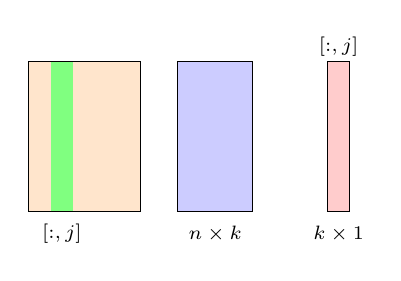
\begin{tikzpicture}[scale=0.95, every node/.style={font=\scriptsize}]
  \draw[fill=orange!20] (0,0) rectangle (1.5,2);
  \fill[green!50] (0.3,0) rectangle (0.6,2);
  \node at (0.45,-0.3) {\scriptsize $\mA[:, j]$};
  \node at (0.75,2.2) {$\mA$};

  \draw[fill=blue!20] (2.0,0) rectangle (3.0,2);
  \node at (2.5,2.2) {$\mW$};
  \node at (2.5,-0.3) {\scriptsize $n \times k$};

  \draw[fill=red!20] (4.0,0) rectangle (4.3,2);
  \node at (4.15,2.2) {$\mH[:, j]$};
  \node at (4.15,-0.3) {\scriptsize $k \times 1$};
\end{tikzpicture}

\textbf{Repeat:} for $j = 0$ to $m - 1$ 

 $\mH[:, j] \leftarrow \text{LS}(\mW, \mA[:, j])$
\end{frame}


\begin{frame}[fragile]{Step 2: Fix $\mH$, Learn $\mW$ One Row at a Time}
\textbf{Goal:} Learn $\mW[i, :] \in \mathbb{R}^{1 \times k}$ row by row.

\textbf{Start from:} $\mA[i, :] \approx \mW[i, :] \cdot \mH$

\textbf{Transpose both sides:}
\begin{equation*}
\mA[i, :]^\top \approx \mH^\top \cdot \mW[i, :]^\top
\end{equation*}

\textbf{Looks like LS again:} $\vy \approx \mX \vtheta$

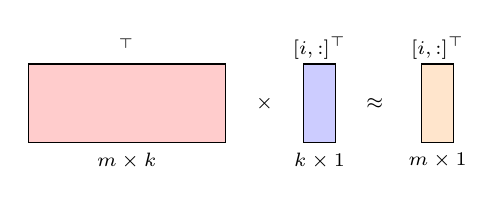
\begin{tikzpicture}[scale=1.0, every node/.style={font=\scriptsize}]
  \draw[fill=red!20] (0,0) rectangle (2.5,1);
  \node at (1.25,1.2) {$\mH^\top$};
  \node[below] at (1.25,0) {\scriptsize $m \times k$};

  \node at (3,0.5) {$\times$};

  \draw[fill=blue!20] (3.5,0) rectangle (3.9,1);
  \node at (3.7,1.2) {$\mW[i, :]^\top$};
  \node[below] at (3.7,0) {\scriptsize $k \times 1$};

  \node at (4.4,0.5) {$\approx$};

  \draw[fill=orange!20] (5.0,0) rectangle (5.4,1);
  \node at (5.2,1.2) {$\mA[i, :]^\top$};
  \node[below] at (5.2,0) {\scriptsize $m \times 1$};
\end{tikzpicture}

\vspace{0.4em}
\textbf{Solve: } $\mW[i, :]^\top \leftarrow \text{LS}(\mH^\top, \mA^\top[:, i])$ for all $i$
\end{frame}


\begin{frame}[fragile]{Final ALS Loop Summary}
\textbf{Repeat for $T$ iterations:}

\vspace{0.5em}
\begin{itemize}
  \item Fix $\mW$, then for each $j$, compute $\mH[:, j] \leftarrow \text{LS}(\mW, \mA[:, j])$
  \item Fix $\mH$, then for each $i$, compute $\mW[i, :]^\top \leftarrow \text{LS}(\mH^\top, \mA^\top[:, i])$
\end{itemize}

\vspace{0.4em}
\textbf{All updates use standard least squares!}

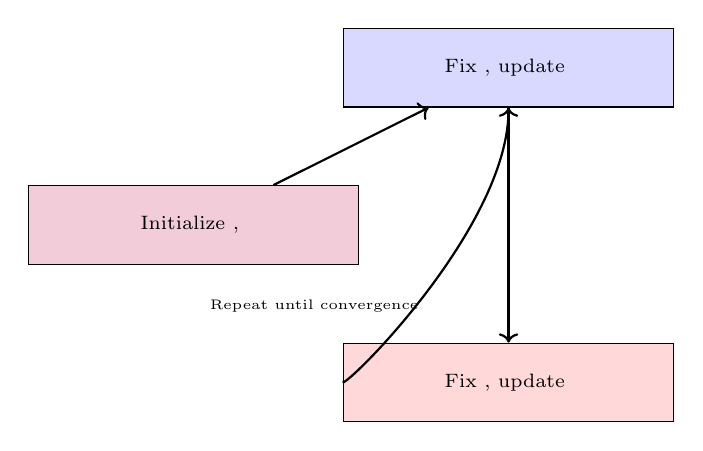
\begin{tikzpicture}[node distance=3.2cm, every node/.style={font=\scriptsize}]
  % Nodes
  \node[draw, fill=purple!20, minimum width=4.2cm, minimum height=1cm, align=center] (init) at (0,0) {Initialize $\mW$, $\mH$};
  \node[draw, fill=blue!15, minimum width=4.2cm, minimum height=1cm, align=center] (fixW) at (4,2) {Fix $\mW$, update $\mH$};
  \node[draw, fill=red!15, minimum width=4.2cm, minimum height=1cm, align=center] (fixH) at (4,-2) {Fix $\mH$, update $\mW$};

  % Arrows
  \draw[->, thick] (init) -- (fixW);
  \draw[->, thick] (fixW) -- (fixH);
  \draw[->, thick] (fixH) .. controls +(left:2cm) and +(down:2cm) .. node[below left, font=\tiny] {Repeat until convergence} (fixW);
\end{tikzpicture}
\end{frame}




\section{Algorithm 2: Gradient Descent}

\begin{frame}{Gradient Descent: Matrix Factorization Setup}
\textbf{Goal:} Find $\mW \in \mathbb{R}^{n \times k}$ and $\mH \in \mathbb{R}^{k \times m}$ such that:
\[
\mA \approx \mW \mH
\]

\vspace{0.5em}
\textbf{Objective Function:}
\[
L(\mW, \mH) = \sum_{(i,j) \in \Omega} (a_{ij} - \vw_i^\top \vh_j)^2
\]

\pause
\textbf{Initialize:}
\begin{itemize}
  \item $\mW$: $n \times k$ matrix with small random values
  \item $\mH$: $k \times m$ matrix with small random values
\end{itemize}

\pause
\textbf{Gradient Descent Loop:}
\begin{itemize}
  \item For $t = 1$ to $T$:
  \begin{itemize}
    \item $\mW \leftarrow \mW - \alpha \cdot \nabla_{\mW} L(\mW, \mH)$
    \item $\mH \leftarrow \mH - \alpha \cdot \nabla_{\mH} L(\mW, \mH)$
  \end{itemize}
\end{itemize}

\pause
\textbf{Note:} Gradients can be computed either over all $(i,j) \in \Omega$ (Batch GD) or stochastically.

\begin{keypointsbox}{}
Gradient descent simultaneously updates \textbf{all} of $\mW$ and $\mH$ based on the total reconstruction error.
\end{keypointsbox}
\end{frame}



\section{Algorithm Comparison and Practical Considerations}

\begin{frame}{ALS vs SGD: Head-to-Head Comparison}
\begin{center}
\renewcommand{\arraystretch}{1.4}
\begin{tabular}{l|cc}
\toprule
\textbf{Aspect} & \textbf{ALS} & \textbf{SGD} \\
\midrule
\textbf{Updates} & Alternating & Simultaneous \\
\textbf{Convergence} & Faster, more stable & Slower, can oscillate \\
\textbf{Parallelization} & Excellent & Limited \\
\textbf{Memory} & Higher & Lower \\
\textbf{Implementation} & Complex & Simple \\
\textbf{Hyperparameters} & Few (rank $r$) & Many ($\alpha$, schedule) \\
\textbf{Scalability} & Very good & Good \\
\bottomrule
\end{tabular}
\end{center}

\pause
\textbf{When to Use Which?}
\begin{itemize}[<+->]
    \item \textbf{ALS:} Large-scale, production systems (Spark, distributed)
    \item \textbf{SGD:} Online learning, real-time updates, research
\end{itemize}
\end{frame}

\begin{frame}{Advanced Considerations: Regularization}
\textbf{Problem:} Basic matrix factorization can overfit to training data

\pause
\textbf{Solution:} Add regularization terms to control complexity
\begin{equation*}
\minimize_{\mW,\mH} \sum_{(i,j) \in \Omega} (a_{ij} - \vw_i^T \vh_j)^2 + \lambda(\|\mW\|_F^2 + \|\mH\|_F^2)
\end{equation*}

\pause
\textbf{What this does:}
\begin{itemize}[<+->]
    \item Penalizes large feature values
    \item Prevents overfitting to observed ratings
    \item $\lambda$ controls regularization strength
    \item Helps generalization to unseen ratings
\end{itemize}
\end{frame}

\begin{frame}{Advanced Considerations: Bias Terms}
\textbf{Real-world insight:} Not all ratings differences are due to preferences!

\pause
\textbf{Bias sources:}
\begin{itemize}[<+->]
    \item \textbf{Global bias $\mu$:} Average rating across all users/movies
    \item \textbf{User bias $b_i$:} Some users rate higher than others
    \item \textbf{Item bias $b_j$:} Some movies are generally better rated
\end{itemize}

\pause
\textbf{Enhanced model:}
\begin{equation*}
\hat{a}_{ij} = \mu + b_i + b_j + \vw_i^T \vh_j
\end{equation*}

\pause
\begin{examplebox}{Example}
Mean rating = 3.5, Arjun rates 0.5 higher, Sholay gets 0.8 higher

$\hat{a}_{\text{Arjun,Sholay}} = 3.5 + 0.5 + 0.8 + \vw_{\text{Arjun}}^T \vh_{\text{Sholay}}$
\end{examplebox}
\end{frame}

\begin{frame}{Advanced Considerations: Implicit Feedback}
\textbf{Beyond explicit ratings:} Many systems have only implicit feedback

\pause
\textbf{Examples of implicit feedback:}
\begin{itemize}[<+->]
    \item User clicked on movie (binary: 0 or 1)
    \item User watched movie for 5 minutes vs 2 hours
    \item User added to watchlist vs ignored
\end{itemize}

\pause
\textbf{Confidence weighting:}
\begin{equation*}
\text{Confidence: } c_{ij} = 1 + \alpha \cdot \text{frequency}_{ij}
\end{equation*}

\pause
\begin{keypointsbox}{}
\textbf{Idea:} More interactions = higher confidence in preference
\end{keypointsbox}
\end{frame}

\begin{frame}{Advanced Considerations: Cold Start Problem}
\textbf{The Challenge:} What about new users or movies with no ratings?

\pause
\textbf{Strategies:}
\begin{itemize}[<+->]
    \item \textbf{Content-based features:} Use movie genres, actors, directors
    \item \textbf{Demographic information:} Age, location, gender of users
    \item \textbf{Hybrid approaches:} Combine collaborative + content-based
    \item \textbf{Popular items:} Recommend trending content initially
\end{itemize}

\pause
\begin{alertbox}{Real-World Solution}
Most production systems use hybrid approaches combining multiple signals
\end{alertbox}
\end{frame}

\section{Hands-On Understanding}

\begin{frame}{Let's Build Intuition: Small Example}
\textbf{Our 3×3 rating matrix:}
\begin{equation*}
\mA = \begin{bmatrix}
5 & ? & 2 \\
4 & 4 & ? \\
? & 5 & 1
\end{bmatrix}
\end{equation*}

\pause
\textbf{Goal:} Find $\mW \in \Real^{3 \times 2}$ and $\mH \in \Real^{2 \times 3}$ such that:
\begin{equation*}
\mA \approx \mW \mH = \begin{bmatrix}
w_{11} & w_{12} \\
w_{21} & w_{22} \\
w_{31} & w_{32}
\end{bmatrix}
\begin{bmatrix}
h_{11} & h_{12} & h_{13} \\
h_{21} & h_{22} & h_{23}
\end{bmatrix}
\end{equation*}

\pause
\textbf{Constraint:} Only minimize error on observed entries!
\end{frame}

\begin{frame}{Step-by-Step ALS Solution}
\textbf{Iteration 1:} Initialize randomly
\begin{equation*}
\mW^{(0)} = \begin{bmatrix} 0.5 & 0.3 \\ 0.4 & 0.6 \\ 0.2 & 0.8 \end{bmatrix}, \quad
\mH^{(0)} = \begin{bmatrix} 1.0 & 0.5 & 0.2 \\ 0.3 & 1.2 & 0.8 \end{bmatrix}
\end{equation*}

\pause
\textbf{Update User 1:} Only use observed ratings (positions 1,3)
\begin{align}
\vy_1 &= [5, 2]^T \\
\mX_1 &= \begin{bmatrix} 1.0 & 0.3 \\ 0.2 & 0.8 \end{bmatrix} \text{ (columns 1,3 of } \mH^{(0)T}\text{)}
\end{align}

\pause
\textbf{Solve:} $\vw_1^{(1)} = \text{LS}(\mX_1, \vy_1)$

Continue for all users and movies...
\end{frame}

\stepcounter{popquiz}
\begin{frame}{Pop Quiz \#\thepopquiz: Netflix Engineering Challenge}
\begin{popquizbox}{\thepopquiz}
You're Netflix's lead ML engineer. You have:
\begin{itemize}
    \item 200M users, 15K movies  
    \item 20B ratings (0.67\% filled)
    \item Need real-time recommendations
    \item New users/movies arrive daily
\end{itemize}

\pause
Design your recommendation system:
\begin{enumerate}[<+->]
    \item Which algorithm: ALS or SGD? Why?
    \item What rank $r$ would you choose?
    \item How to handle new users?
    \item How to handle the scale?
\end{enumerate}

\pause
\textbf{Suggested Solution:}
\begin{itemize}
    \item \textbf{ALS} for batch processing (Spark), \textbf{SGD} for online updates
    \item $r = 50-200$ (balance between expressiveness and efficiency)
    \item Hybrid: Content-based for cold start + collaborative filtering
    \item Distributed computing, approximate algorithms, caching
\end{itemize}
\end{popquizbox}
\end{frame}

\section{Summary and Key Takeaways}

\begin{frame}{Key Insights: Part 1}
\begin{enumerate}[<+->]
    \item \textbf{Sparsity $\Rightarrow$ Factorization}: Sparse matrices can be approximated by low-rank factorizations
    
    \item \textbf{Latent Features}: Users and items characterized by hidden factors
    
    \item \textbf{Bilinear Problem}: Non-convex jointly, convex individually
\end{enumerate}
\end{frame}

\begin{frame}{Key Insights: Part 2}  
\begin{enumerate}[<+->]
    \setcounter{enumi}{3}
    \item \textbf{Scale Matters}: Algorithm choice depends on data size
    
    \item \textbf{Real-World Complexity}: Need regularization, bias terms, cold start solutions
\end{enumerate}

\pause
\textbf{The Mathematical Beauty:}
\begin{equation*}
\boxed{\text{Collaborative Filtering} = \text{Matrix Factorization} = \text{Dimensionality Reduction}}
\end{equation*}
\end{frame}

\begin{frame}{Extensions: Interpretable Factorization}
\textbf{Non-negative Matrix Factorization (NMF):}

\pause
\begin{definitionbox}{NMF Constraint}
All factors must be non-negative: $\mW \geq 0, \mH \geq 0$
\end{definitionbox}

\pause
\textbf{Why this matters:}
\begin{itemize}[<+->]
    \item Factors represent "parts" or "components"
    \item No negative contributions → interpretable
    \item Example: Genre weights are always positive
\end{itemize}

\pause
\begin{examplebox}{Movie Example}
If factor 1 = "Action-ness", then $h_{1j} \geq 0$ means movie $j$ has some amount of action (never "negative action")
\end{examplebox}
\end{frame}

\begin{frame}{Extensions: Deep Learning Approaches}
\textbf{Deep Matrix Factorization:}

\pause
\textbf{Limitation of linear factorization:}
$$\hat{a}_{ij} = \vw_i^T \vh_j \text{ (only linear interactions)}$$

\pause
\textbf{Deep learning solution:}
$$\hat{a}_{ij} = f_{\text{NN}}(\vw_i, \vh_j)$$
where $f_{\text{NN}}$ is a neural network

\pause
\begin{keypointsbox}{}
Captures complex, non-linear user-item interaction patterns!
\end{keypointsbox}

\pause
\textbf{Examples:}
\begin{itemize}[<+->]
    \item Neural Collaborative Filtering
    \item AutoRec (Autoencoder-based)
    \item Deep Factorization Machines
\end{itemize}
\end{frame}

\begin{frame}{Extensions: Advanced Interaction Modeling}
\textbf{Factorization Machines:} Handle multi-way interactions

\pause
\begin{examplebox}{Beyond User-Movie}
Traditional: User × Movie

FM: User × Movie × Time × Device × Location × Weather
\end{examplebox}

\pause
\begin{keypointsbox}{}
Enable richer context-aware recommendations
\end{keypointsbox}
\end{frame}

\begin{frame}{Extensions: Neural Approaches}
\textbf{Variational Autoencoders:}
\begin{itemize}[<+->]
    \item Probabilistic approach with uncertainty estimates
    \item Can generate diverse, novel recommendations
\end{itemize}

\pause
\textbf{Graph Neural Networks:}
\begin{itemize}[<+->]
    \item Model interactions as graph structure
    \item Examples: GraphRec, NGCF, LightGCN
\end{itemize}
\end{frame}

\begin{frame}{Extensions: Exploration and Real-World Applications}
\textbf{Multi-armed Bandits:} Balance exploration vs exploitation

\pause
\begin{alertbox}{The Dilemma}
Recommend known good items vs explore new possibilities?
\end{alertbox}

\pause
\begin{keypointsbox}{}
Balance accuracy with discovery!
\end{keypointsbox}
\end{frame}

\begin{frame}{Real-World Applications}
\textbf{Matrix factorization is everywhere:}

\pause
\begin{itemize}[<+->]
    \item \textbf{E-commerce:} Amazon recommendations
    \item \textbf{Music streaming:} Spotify Discover Weekly
    \item \textbf{Social media:} Facebook friend suggestions
    \item \textbf{Advertising:} Targeted ads
\end{itemize}

\pause
\begin{keypointsbox}{}
Same principles apply across domains!
\end{keypointsbox}
\end{frame}

\stepcounter{popquiz}
\begin{frame}{Pop Quiz \#\thepopquiz: Matrix Factorization Fundamentals}
\begin{popquizbox}{\thepopquiz}
\textbf{True or False?}

\begin{enumerate}
    \item Matrix factorization can only work with explicit ratings
    \item ALS always converges to the global optimum
    \item A rank-1 factorization means all users have identical preferences
\end{enumerate}
\end{popquizbox}
\end{frame}

\begin{frame}{Pop Quiz \#\thepopquiz: Answers - Fundamentals}
\begin{popquizbox}{\thepopquiz}
\textbf{Answers:}

\begin{enumerate}
    \item \textbf{False} - Works with implicit feedback too
    \item \textbf{False} - Converges to local optimum only  
    \item \textbf{False} - Rank-1 means one pattern, not identical
\end{enumerate}
\end{popquizbox}
\end{frame}

\stepcounter{popquiz}
\begin{frame}{Pop Quiz \#\thepopquiz: Advanced Topics}
\begin{popquizbox}{\thepopquiz}
\textbf{True or False?}

\begin{enumerate}
    \item Adding regularization always improves recommendations
    \item SGD is better than ALS for all applications
\end{enumerate}

\textbf{Bonus:} What are the main trade-offs between ALS and SGD?
\end{popquizbox}
\end{frame}

\begin{frame}{Pop Quiz \#\thepopquiz: Answers - Advanced Topics}
\begin{popquizbox}{\thepopquiz}
\textbf{Answers:}

\begin{enumerate}
    \item \textbf{False} - Too much regularization causes underfitting
    \item \textbf{False} - Choice depends on data scale and needs
\end{enumerate}

\textbf{Bonus:} \textbf{ALS:} Fast, parallel. \textbf{SGD:} Online, low memory.
\end{popquizbox}
\end{frame}





\end{document}